\documentclass{sig-alternate}
\usepackage{listings}
\begin{document}
\conferenceinfo{CSC766}{'15 Spring Raleigh, North Carolina USA}

\title{Ontology-based Knowledge Representation for PORPLE}
\subtitle{[CSC766 Final Report]}

\numberofauthors{3}
\author{
\alignauthor
Feifei Wang\\
       \affaddr{North Carolina State University}\\
       \email{fwang12@ncsu.edu}
\alignauthor
Yue Zhao\\
       \affaddr{North Carolina State University}\\
       \email{yzhao30@ncsu.edu}
\alignauthor
Xipeng Shen\\
       \affaddr{North Carolina State University}\\
       \email{xshen5@ncsu.edu}
}
\maketitle
\begin{abstract}
Data placement is important for the performance of a GPU (Graphic Processing Unit) program. However, where to place the data is a complex decision for a programmer to make. Among the recent techniques in solving data placement problem, PORPLE is a representative one. PORPLE is a portable data placement engine that uses hardware information (memory systems and processors) described by memory specification language (MSL) and software information (data access patterns) gathered from a compiler called PORPLE-C. Because of the two different representations, it is hard to share common understanding of the program, and reuse information. Providing a more general, uniform and reusable representation can make data replacement decisions more efficient, interoperable and reusable.

In this paper, we apply ontology-based techniques to systematically and formally represent both hardware information and software information used by PORPLE hoping to achieve efficiency, interoperability and reusability. Specifically, we transform the information of GPU memory systems and processors, and the data access patterns gathered by PROPLE-C to ontology which can be used by PORPLE for data replacement.
 
\end{abstract}

\terms{Compiler}

\keywords{compiler, ontology, data placement}

\section{Introduction}
Data placement is essential for the performance of a GPU (Graphic Processing Unit) program \cite{related1}. However, where to place the data depends on the hardware information of the GPU and software information of the program and its input. The hardware information of the GPU includes its memory systems and processors, while the software information means the data access patterns associated with the input to the programs. The memory systems of GPUs are becoming increasingly complex. For example, there exists more than eight types of memory (including caches) on the Tesla M2075 GPU. These memories have different size limitations, block sizes, access constraints and etc. Also, the suitable placements depend on the program inputs since different inputs to a program may lead to different data access patterns, and thus require different data placement. As a result, data placement problem is difficult but should be solved.

There have been some efforts to address the data placement problem \cite{related1, related2, related3, porple}. Among them, PORPLE \cite{porple} is a representative one since it considers various types of GPU programs. PORPLE is a portable data placement engine that takes both hardware information (memory systems and processors) and software information (data access patterns) into consideration and use them to make data placement decisions. PORPLE obtains information about memory systems and processors from memory specification language (MSL), and uses the runtime profiling to acquire the data access patterns. In such a sense, PORPLE uses two different types of representations, which makes it hard to share common understanding of the program and reuse information. Providing a more general, uniform and reusable representation can improve the efficiency, interoperability and reusability of PORPLE and potentially some other work.

There exists various techniques to represent knowledge \cite{intro2}. Recently, ontology-based knowledge bases are becoming increasingly popular. Ontology is a general-purpose modeling for knowledge resources used to define a common vocabulary and a shared understanding explicitly \cite{ontology1, ontology2}. It has been successfully used to build knowledge bases in many fields \cite{ontology3, ontology4, ontology5, ontology6, work1, work2}. Motivated by their advances, we choose ontology as the representation.

In this paper, we apply ontology-based techniques to systematically and formally represent both hardware information and software information hoping to make PORPLE more efficient, interoperable and reusable. Specifically, we transform the information of GPU memory systems and processors, and the data access patterns gathered to ontology which can be used by PORPLE for data replacement. Note that although our work is applied to PORPLE, it can also be applied to other work.

This paper is organized as follows. In Section 2, we present the motivation of our work. Section 3 illustrates the challenges of the project, our solutions, and lessons we learned. In Section 4 we explain our methodology in detail. Section 5 shows the results. Section 6 concludes this paper and discusses some possible future work.

\section{Motivation}
This work is mainly motivated by an observation that PORPLE uses two different representations for hardware information and software information. Hardware information is represented by memory specification language (MSL), which is a carefully designed small specification language. It describes the memory systems of a GPU. \ref{fig:msl} shows the MSL specification of the Tesla M2075 GPU as an example. The MSL describes the properties of a type of memory and its relations with other pieces of memory in a system. For example, the second line of the file shows the properties of globalMem. The name of the memory is globalMem, its id is 8, it is software manageable, allows read and write accesses, and etc. It also shows the relations between globalMem and L2 is that globalMem has an upper level called L2. Software information, which is data access patterns, is represented by a form defined by Chen et al. \cite{porple} \ref{fig:dap} presents one data access pattern used by PORPLE. In this file, the second line shows that the total memory access time is 64, L1 cache hit is 0, and L2 cache hit is 0.

Due to the two different representations, it is hard for them to share common understanding of the program and reuse information. In such a sense, we are motivated to choose ontology as a more general, uniform and reusable representation hoping to improve the efficiency, interoperability and reusability of PORPLE and potentially some other work.

This work is also motivated by the success of some previous work of using ontology to systematically represent, reuse, and manipulate software information, hardware information and optimization information. For example, OpenK adapts ontology-based techniques to build open and reusable knowledge bases to do program analysis and optimization in HPC. Sosnovsky et al. \cite{work1} and Ganapathi \cite{work2} et al. use ontology to teach abstract programming language. Moor et al. \cite{ontology3} and Leenheer et al. \cite{ontology4} focus on community-based evolution of knowledge-intensive systems with ontology. Tang et al. \cite{ontology5} implement a profile compiler that support ontology-based, community-grounded, multilingual, collaborative group decision making by leveraging ontology. 

\begin{figure*}
\centering
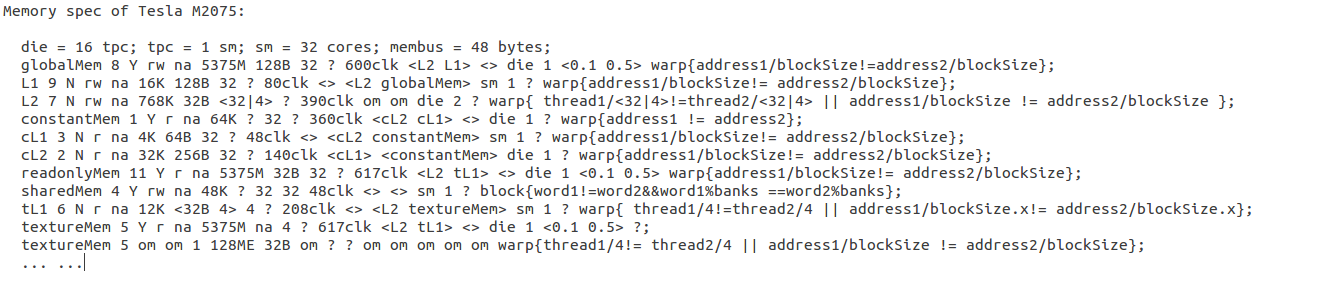
\epsfig{file=msl.png,height=4cm}
\caption{The memory specification of Tesla M2075 in MSL}
\label{fig:msl}
\end{figure*}

\begin{figure}
\centering
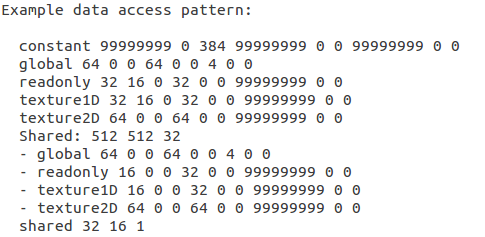
\epsfig{file=dap.png,height=4cm}
\caption{The data access pattern used by PORPLE}
\label{fig:dap}
\end{figure}

\section{Challenge, Solution and Lesson}
Transforming MSL and data access patterns used by PORPLE to ontolgoy is quite straightforward. The main challenge is to understand ontology. In this section, we introduce the challenge to understand ontology, how we overcome them, and the lessons we learned.

\subsection{Challenge}
Ontologies have three parts: individuals, properties and classes \cite{what1}. Individuals are objects in the domain in which we are interested. Properties represent binary relations between two individuals. Objects with similar characteristics are grouped by classes. In this part we use \ref{fig:msl} as an example to illustrate the challenges. 

The individual part is related easy to understand. We just use 

Each object property may have a corresponding inverse property. If some property links individual a to individual b then its inverse property will link individual b to individual a. For example, Figure 4.16 shows the property hasParent and its inverse property hasChild — if Matthew hasParent Jean, then because of the inverse property we can infer that Jean hasChild Matthew.

Datatype properties describe relationships between individuals and data values. Object properties describe relationships between two individuals.
Datatype properties link an individual to an XML Schema Datatype value or an rdf literal. In other words, they describe relationships between an individual and data values. 

OWL allows us to define individuals and to assert properties about them. Individuals can also be used in class descriptions, namely in hasValue restrictions and enumerated classes which will be explained in section 7.2 and section 7.3 respectively. To create individuals in Prot ́eg ́e 4 the ‘Individuals Tab’ is used.
Suppose we wanted to describe the country of origin of various pizza toppings. We would first need to add various ‘countries’ to our ontology. Countries, for example, ‘England’, ‘Italy’, ‘America’, are typically thought of as being individuals (it would be incorrect to have a class England for example, as it’s members would be deemed to be, ‘things that are instances of England’). To create this in our Pizza Ontology we


OWL object property characteristics:
If a property is functional, for a given individual, there can be at most one individual that is related to the individual via the property. 
If a property is inverse functional then it means that the inverse property is functional. 
If a property is transitive, and the property relates individual a to individual b, and also individual b to individual c, then we can infer that individual a is related to individual c via property P. 
If a property P is symmetric, and the property relates individual a to individual b then individual b is also related to individual a via property P.
If a property P is asymmetric, and the property relates individual a to individual b then individual b cannot be related to individual a via property P. 
Reflexive properties
Irreflexive properties

Properties may have a domain and a range specified. Properties link individuals from the domain to individuals from the range. 



how to develop an ontology?
defining concepts in the domain (classes)
arranging the concepts in a hierarchy (subclass-superclass hierarchy) -- I don't have this in project
Defining which attributes and properties (slots) classes can have and constraints on their values
Defining individuals and filling in slot values

what is the domain that the ontology will cover? for what we are going to use the ontology? for what types of questions the information in the ontology should provide answers?
which characteristics should I consider when choosing ...?
what are the terms we need to talk about?
what are the properties of these terms?
what do we want to say about the terms?

enumerat terms... define classes and the class hierarchy... define properties of classes ... valuetype .. value...
The ClassAssertion axiom allows one to state that an individual is an instance of a particular class.
The ObjectPropertyAssertion axiom allows one to state that an individual is connected by an object property expression to an individual
The DataPropertyAssertion axiom allows one to state that an individual is connected by a data property expression to a literal

Individuals in the OWL 2 syntax represent actual objects from the domain. There are two types of individuals in the syntax of OWL 2. Named individuals are given an explicit name that can be used in any ontology to refer to the same object. Anonymous individuals do not have a global name and are thus local to the ontology they are contained in.


The sentence "The individual I is an instance of the class C" can be understood as a statement that I is an instance of the UML class Individual, C is an instance of the UML class Class, and there is an instance of the UML class ClassAssertion that connects I with C. This statement can be captured precisely using the structural specification as ClassAssertion( C I ).

The individual a:Peter can be used to represent a particular person. It can be used in axioms such as the following one:

ClassAssertion( a:Person a:Peter )	Peter is a person.

DataPropertyAssertion( a:hasAge a:Meg "17"^^xsd:double )	Meg is seventeen years old.
The first axiom states that all values of the a:hasAge property must be in the value space of xsd:integer, but the second axiom provides a value for a:hasAge that is equal to the floating-point number 17. Since floating-point numbers are not contained in the value space of xsd:integer, the mentioned ontology is inconsistent.

bjectPropertyAssertion( a:hasBrother a:Chris a:Stewie )	Stewie is a brother of Chris.

http://protege.stanford.edu/publications/ontology_development/ontology101.html

\subsection{Solution}

\subsection{Lessons}

\section{Methodology}

\section{Results}

\section{Conclusion and Future Work}




Classes can be organized into superclass-subclass hierarchy and they are described or defined by the relationships that individuals participate in.

\begin{table*}

\centering

\caption{Correctness for All the Questions}

\begin{tabular}{|l|l|} \hline

% & \multicolumn{4}{l|}{forward questions} & \multicolumn{4}{l|}{backward questions} & \multicolumn{4}{l|}{same-different questions}\\ \hline

Classes and Instances&ClassAssertion()\\ \hline
Class Hierarchies&SubClassOf()\\ \hline
Object Properties&ObjectPropertyAssertion()\\ \hline
Property Hierarchies&SubObjectPropertyOf()\\ \hline
Datatypes&DataPropertyAssertion()\\ \hline
\end{tabular}
\label{table:accuracy}
\end{table*}

\section{Acknowledgments}
This section is optional; it is a location for you
to acknowledge grants, funding, editing assistance and
what have you.  In the present case, for example, the
authors would like to thank Gerald Murray of ACM for
his help in codifying this \textit{Author's Guide}
and the \textbf{.cls} and \textbf{.tex} files that it describes.


\bibliographystyle{abbrv}
\bibliography{sigproc} 
\subsection{References}
Generated by bibtex from your ~.bib file.  Run latex,
then bibtex, then latex twice (to resolve references)
to create the ~.bbl file.  Insert that ~.bbl file into
the .tex source file and comment out
the command \texttt{{\char'134}thebibliography}.

\end{document}
\begin{thebibliography}{1}

\bibitem{ontology1}
T.~R. Gruber.
\newblock Toward principles for the design of ontologies used for knowledge
sharing?
\newblock {\em International journal of human-computer studies},
43(5):907--928, 1995.

\end{thebibliography}
